
\documentclass[a4paper, 12pt, english]{article}

\usepackage{babel}
\usepackage[utf8]{inputenc}
\usepackage{enumitem}
\usepackage[T1]{fontenc}
\usepackage{amsmath}
\usepackage{amssymb}
\usepackage{amsthm}
\usepackage{wasysym}
\usepackage{listings}
\usepackage{graphicx}
\usepackage{icomma}
\usepackage{hyperref}

\newcommand{\sijoitus}[2]%
{\operatornamewithlimits{\Bigl/}_{\!\!\!#1}^{\,#2}}
\setcounter{MaxMatrixCols}{20}
\newcommand{\R}{\mathbb{R}}
\newcommand{\C}{\mathbb{C}}
\newcommand{\Z}{\mathbb{Z}}
\newcommand{\Q}{\mathbb{Q}}
\newcommand{\N}{\mathbb{N}}
\newcommand{\ysumma}{\overline{\mathrm{S}}}
\newcommand{\asumma}{\underline{\mathrm{S}}}
\newcommand{\nolv}{\underline{0}}
\newcommand{\cl}[1]{\overline{#1}}

\title{Blue algae project report}
\author{Nadezhda Novikovskaia, Ossi Räisä, Janani Subramanian}

\begin{document}
\maketitle

\section{Data}

\subsection{Healthcare visits}
The healthcare visits data was downloaded from
the THL
\href{https://sampo.thl.fi/pivot/prod/fi/avopika/pikarap01/fact_ahil_pikarap01.csv?row=palveluntuottaja-349235L&column=viikko-349531L}{API}.
The API return logged visits to healthcare providers for each week
of 2018 and 2019 (until week 38). To find to locations of the providers,
a list of subproviders with their municipalities was used. We assumed
that each provider is in the municipality where most of their
subproviders are. Then the providers were grouped by their municipality
and the groups were summed with missing values assumed to be zeros
giving healthcare visits for each municipality for each week.

\subsection{Algae}
The algae data is from an API used by the
\href{https://www.jarviwiki.fi/wiki/Toiminnot:Semanttinen_kysely/Lev%C3%A4taulukko}
{Lake and Sea wiki algae table page}.
The URL for the API was found by looking at the requests made by
the page and finding the request returning the algae data.

The API returns the data as a json string containing a list of
measurements. From each measurement the date, place and algae level were
extracted. The measurements were first compiled to a table with weeks
as columns, measurement stations as rows and algae levels as values.
There was mostly one measurement per week for each station, so the
few conflicting measurements for were ignored. Then the stations
were grouped by their municipality and the algea levels of each group
were averaged, giving a table with municipalities as rows.

The algae level is a number from 0 to 3 where 0 is no algae
and 3 is the most algae. The time period is weeks from 23 to 39
in 2018 and 23 to 37 in 2019.
The data has a lot of missing values, even for municipalities.

\subsection{Weather and airquality}
The weather and airquality data was downloaded from the
\href{https://ilmatieteenlaitos.fi/tallennetut-kyselyt}{WFS API}
of the Finnish Meteorological Institute.
The airquality is from the stored query
\mbox{``urban::observations::airquality::hourly::timevaluepair''}
and the rain and temperature is from
\mbox{``fmi::observations::weather::daily::timevaluepair''}.
As the airquality returns hourly data getting all of it
for two years takes over a hundred queries,
it and the weather data was only retrieved for
municipalities with no missing algae values and
a population over 10 000 people. The airquality data includes
several measures for different substances that
pollute the air and an index, which was the only value
we used.

The airquality, temperature and rain values for were
grouped by the week and year they are from and
averaged. There were 22 municipalities that had the
algae, weather and airquality data and were large
enough.

\subsection{Population}
The population data was downloaded from Statistics Finland interface services
``Municipal key figures'' (2018 population) and
``Preliminary population structure by area'' (2019 population).

\section{Analysis}
To predict healthcare visits we made the data into a
single table where each row is a single week of one
municipality. The columns are the algae, temperature,
rain and airquality values for that week and several
previous weeks, the number of which was varied.
The table also had the population of the municipality
for the row's year and finally the number of healthcare
visits for the week and municipality.

At first we ran linear regression, random forest regression
and support vector machine regression on the data for just
one municipality without population. The results were not good,
so we included more municipalities and their population.
This had better results. The numbers shown on the
pitch were with 6 municipalities. After the pitch we
downloaded the weather and airquality data for
the rest of the municipalities and ran the regression
methods. As the SVM was not performing well it was
replaced by a decision tree.

The first experiement has a total of 4 weeks for
each of the features varying with time and the
population, for a total of
17 features. With 22 cities the dataset has 1980 rows.
The random forest has 100 trees with 10 maximum depth
and the decision tree has 3 maximum depth to allow
inspecting it. The next table shows the results.\\

\begin{tabular}{l l l}
Model & Training \(R^2\) & Test \(R^2\) \\
Linear Regression & 0.783 & 0.794 \\
Random Forest & 0.955 & 0.950 \\
Decision Tree & 0.911 & 0.922 \\
\end{tabular}
\\

Surprisingly even the very simple decision tree
gets a high score.
Figure \ref{tree1} shows the decision tree. As we can see
X[16], that being the population, is used in almost
all of the nodes. The linear regression coefficients
are -701, -919,  151 and -340 for the algae on weeks
0, -1, -2, and -3 respectively, 0.24 for population
and 0 for the rest. The algae coefficients are larger
than the population because because the algae level is from 0 to 3
while the population is over 10 000.

This means that the population actually
explain most of the healthcare visits, which is
to be expected. To if the other features are useful at all
for the next experiement we removed all features
except population. Model parameters were not changed.
The next table shows the results.\\

\begin{tabular}{l l l}
Model & Training \(R^2\) & Test \(R^2\) \\
Linear Regression & 0.783 & 0.794 \\
Random Forest & 0.944 & 0.949 \\
Decision Tree & 0.910 & 0.920 \\
\end{tabular}
\\

The test scores show very minor drops for random forest
and decision tree and no change for linear regression,
meaning that the other features are not very useful
in the prediction.

For the final experiement we replaces healthcare
visits with visits per population and
removed population from the features.
The table shows the scores.\\

\begin{tabular}{l l l}
Model & Training \(R^2\) & Test \(R^2\) \\
Linear Regression & 0.017 & -0.003 \\
Random Forest & 0.097 & -0.021 \\
Decision Tree & 0.026 & -0.001 \\
\end{tabular}
\\

The scores are very bad so the features are not able
to predict the healthcare visits per population.
As the training score is low even for
the random forest we tried increasing the maximum depth of
the it which, but it did not change the scores significantly.


\begin{figure}
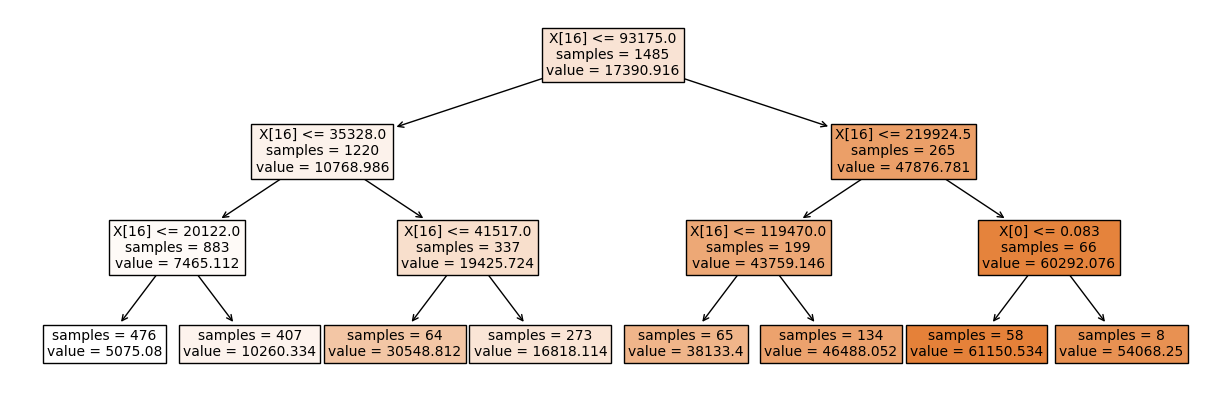
\includegraphics[width=\textwidth]{tree1}
\caption{
X[16] is the population and X[0] is the algae level for the week in question.
Most nodes only use the population.
}
\label{tree1}
\end{figure}


\end{document}
